\documentclass{article}

\usepackage{hyperref}
\hypersetup{
	colorlinks=true,
	linkcolor=blue,
	urlcolor=cyan,}
\usepackage{booktabs}
\usepackage{textgreek}
\usepackage{gensymb}

%%%%%%%%%%%%%%%%%%%%%%%%%%%%%%%%%%%%%%%%%
% Lachaise Assignment
% Structure Specification File
% Version 1.0 (26/6/2018)
%
% This template originates from:
% http://www.LaTeXTemplates.com
%
% Authors:
% Marion Lachaise & François Févotte
% Vel (vel@LaTeXTemplates.com)
%
% License:
% CC BY-NC-SA 3.0 (http://creativecommons.org/licenses/by-nc-sa/3.0/)
% 
%%%%%%%%%%%%%%%%%%%%%%%%%%%%%%%%%%%%%%%%%

%----------------------------------------------------------------------------------------
%	PACKAGES AND OTHER DOCUMENT CONFIGURATIONS
%----------------------------------------------------------------------------------------

\usepackage{amsmath,amsfonts,stmaryrd,amssymb} % Math packages

\usepackage{enumerate} % Custom item numbers for enumerations

\usepackage[ruled]{algorithm2e} % Algorithms

\usepackage[framemethod=tikz]{mdframed} % Allows defining custom boxed/framed environments

\usepackage{listings} % File listings, with syntax highlighting
\lstset{
	basicstyle=\ttfamily, % Typeset listings in monospace font
}

%----------------------------------------------------------------------------------------
%	DOCUMENT MARGINS
%----------------------------------------------------------------------------------------

\usepackage{geometry} % Required for adjusting page dimensions and margins

\geometry{
	paper=a4paper, % Paper size, change to letterpaper for US letter size
	top=2.5cm, % Top margin
	bottom=3cm, % Bottom margin
	left=2.5cm, % Left margin
	right=2.5cm, % Right margin
	headheight=14pt, % Header height
	footskip=1.5cm, % Space from the bottom margin to the baseline of the footer
	headsep=1.2cm, % Space from the top margin to the baseline of the header
	%showframe, % Uncomment to show how the type block is set on the page
}

%----------------------------------------------------------------------------------------
%	FONTS
%----------------------------------------------------------------------------------------

\usepackage[utf8]{inputenc} % Required for inputting international characters
\usepackage[T1]{fontenc} % Output font encoding for international characters

\usepackage{XCharter} % Use the XCharter fonts

%----------------------------------------------------------------------------------------
%	COMMAND LINE ENVIRONMENT
%----------------------------------------------------------------------------------------

% Usage:
% \begin{commandline}
%	\begin{verbatim}
%		$ ls
%		
%		Applications	Desktop	...
%	\end{verbatim}
% \end{commandline}

\mdfdefinestyle{commandline}{
	leftmargin=10pt,
	rightmargin=10pt,
	innerleftmargin=15pt,
	middlelinecolor=black!50!white,
	middlelinewidth=2pt,
	frametitlerule=false,
	backgroundcolor=black!5!white,
	frametitle={Command Line},
	frametitlefont={\normalfont\sffamily\color{white}\hspace{-1em}},
	frametitlebackgroundcolor=black!50!white,
	nobreak,
}

% Define a custom environment for command-line snapshots
\newenvironment{commandline}{
	\medskip
	\begin{mdframed}[style=commandline]
}{
	\end{mdframed}
	\medskip
}

%----------------------------------------------------------------------------------------
%	FILE CONTENTS ENVIRONMENT
%----------------------------------------------------------------------------------------

% Usage:
% \begin{file}[optional filename, defaults to "File"]
%	File contents, for example, with a listings environment
% \end{file}

\mdfdefinestyle{file}{
	innertopmargin=1.6\baselineskip,
	innerbottommargin=0.8\baselineskip,
	topline=false, bottomline=false,
	leftline=false, rightline=false,
	leftmargin=2cm,
	rightmargin=2cm,
	singleextra={%
		\draw[fill=black!10!white](P)++(0,-1.2em)rectangle(P-|O);
		\node[anchor=north west]
		at(P-|O){\ttfamily\mdfilename};
		%
		\def\l{3em}
		\draw(O-|P)++(-\l,0)--++(\l,\l)--(P)--(P-|O)--(O)--cycle;
		\draw(O-|P)++(-\l,0)--++(0,\l)--++(\l,0);
	},
	nobreak,
}

% Define a custom environment for file contents
\newenvironment{file}[1][File]{ % Set the default filename to "File"
	\medskip
	\newcommand{\mdfilename}{#1}
	\begin{mdframed}[style=file]
}{
	\end{mdframed}
	\medskip
}

%----------------------------------------------------------------------------------------
%	NUMBERED QUESTIONS ENVIRONMENT
%----------------------------------------------------------------------------------------

% Usage:
% \begin{question}[optional title]
%	Question contents
% \end{question}

\mdfdefinestyle{question}{
	innertopmargin=1.2\baselineskip,
	innerbottommargin=0.8\baselineskip,
	roundcorner=5pt,
	nobreak,
	singleextra={%
		\draw(P-|O)node[xshift=1em,anchor=west,fill=white,draw,rounded corners=5pt]{%
		Question \theQuestion\questionTitle};
	},
}

\newcounter{Question} % Stores the current question number that gets iterated with each new question

% Define a custom environment for numbered questions
\newenvironment{question}[1][\unskip]{
	\bigskip
	\stepcounter{Question}
	\newcommand{\questionTitle}{~#1}
	\begin{mdframed}[style=question]
}{
	\end{mdframed}
	\medskip
}

%----------------------------------------------------------------------------------------
%	WARNING TEXT ENVIRONMENT
%----------------------------------------------------------------------------------------

% Usage:
% \begin{warn}[optional title, defaults to "Warning:"]
%	Contents
% \end{warn}

\mdfdefinestyle{warning}{
	topline=false, bottomline=false,
	leftline=false, rightline=false,
	nobreak,
	singleextra={%
		\draw(P-|O)++(-0.5em,0)node(tmp1){};
		\draw(P-|O)++(0.5em,0)node(tmp2){};
		\fill[black,rotate around={45:(P-|O)}](tmp1)rectangle(tmp2);
		\node at(P-|O){\color{white}\scriptsize\bf !};
		\draw[very thick](P-|O)++(0,-1em)--(O);%--(O-|P);
	}
}

% Define a custom environment for warning text
\newenvironment{warn}[1][Warning:]{ % Set the default warning to "Warning:"
	\medskip
	\begin{mdframed}[style=warning]
		\noindent{\textbf{#1}}
}{
	\end{mdframed}
}

%----------------------------------------------------------------------------------------
%	INFORMATION ENVIRONMENT
%----------------------------------------------------------------------------------------

% Usage:
% \begin{info}[optional title, defaults to "Info:"]
% 	contents
% 	\end{info}

\mdfdefinestyle{info}{%
	topline=false, bottomline=false,
	leftline=false, rightline=false,
	nobreak,
	singleextra={%
		\fill[black](P-|O)circle[radius=0.4em];
		\node at(P-|O){\color{white}\scriptsize\bf i};
		\draw[very thick](P-|O)++(0,-0.8em)--(O);%--(O-|P);
	}
}

% Define a custom environment for information
\newenvironment{info}[1][Info:]{ % Set the default title to "Info:"
	\medskip
	\begin{mdframed}[style=info]
		\noindent{\textbf{#1}}
}{
	\end{mdframed}
}
 % Include the file specifying the document structure and custom commands

%----------------------------------------------------------------------------------------
%	ASSIGNMENT INFORMATION
%----------------------------------------------------------------------------------------

\title{Week 9: Pulmonary Function (PF) II}
\author{BIOE 320 Systems Physiology Laboratory} 
\date{}
%----------------------------------------------------------------------------------------

\begin{document}
\large
\maketitle

\section*{Objectives}
\begin{enumerate}
	\item To perform mass balances on O\textsubscript{2} and CO\textsubscript{2} during respiration.
	\item To calculate alveolar and pulmonary ventilation rates.
	\item To obtain a value for VO\textsubscript{2}, the volume of oxygen consumed at STP per 1 minute interval, at rest, after exercise, and during hyperventilation.
\end{enumerate}

\section*{Background}
\subsection*{Dead Space}
Defined as the volume of gas that does not participate in gas exchange.
\begin{itemize}
	\item Anatomical dead space (about 150 mL) results from the dead space in the conducting airways (trachea, bronchi, and bronchioles). The air in the conducting airways does not reach the alveoli and, as a result, does not participate in gas exchange.
	\item Alveolar dead space (very small in healthy subjects) results from poor perfusion to the alveoli. When blood perfusion is limited, some alveoli (even when they contain air) will not participate in gas exchange.
	\item Physiological dead space is the sum of the anatomical and alveolar dead space and it represents the volume of air that is inspired but does not participate in gas exchange with blood flowing through the lungs.
\end{itemize}

\subsection*{Ventilation Rate}
Defined as the number of breaths in a given time:
\begin{itemize}
	\item Pulmonary or minute ventilation rate represents the volume of air breathed in and out in one minute.
	\item Alveolar ventilation rate represents the volume of air that reaches the alveoli and is available for gas exchange in 1 minute.
\end{itemize}

\subsection*{Gas Exchange}
The goal of breathing is to provide a continuous supply of O\textsubscript{2} to the tissues and to constantly remove CO\textsubscript{2}. This gas exchange at both the pulmonary and the tissue capillary levels involves simple passive diffusion of O\textsubscript{2} and CO\textsubscript{2} down partial pressure gradients.\\

Atmospheric air is a mixture of gases (about 79\% nitrogen and 21\% oxygen, with almost negligible percentages of CO\textsubscript{2}, water vapor, other gases, and pollutants. Altogether, these gases exert a total atmospheric pressure of 760 mmHg at sea level. This total pressure is equal to the sum of the pressures that each gas in the mixture partially contributes. The pressure exerted by a particular gas is directly proportional to the percentage of that gas in the total air mixture. For example, the partial pressure (or the individual pressure exerted by a gas within a mixture of gases) of oxygen (P\textsubscript{O2}) in atmospheric air is normally 160 mmHg, whereas the atmospheric partial pressure of CO\textsubscript{2} (P\textsubscript{CO2}) is 0.03 mmHg. Since there is a difference in partial pressures between alveolar air and pulmonary capillary blood (e.g. P\textsubscript{O2, alveoli} > P\textsubscript{O2, blood}), gas will diffuse down its partial pressure gradient from the area of higher partial pressure to the area of lower partial pressure (Fig. \ref{partial}).

\begin{figure}[h]
\centering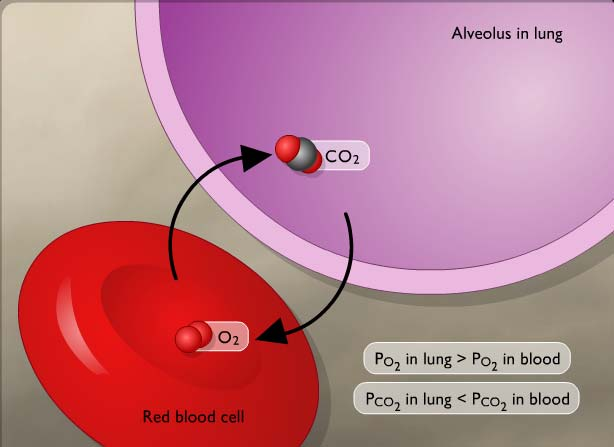
\includegraphics[width=0.6\textwidth]{../images/PF_II_1.jpg}
\caption{Gas exchange in the lungs}
\label{partial}
\end{figure}

In addition to partial pressure gradients, there are several factors that can influence the rate of gas transfer:
\begin{itemize}
	\item \textbf{Surface area}: An increase in surface area of the alveolar membrane will result in an increased rate of transfer. Surface area remains fairly constant under resting conditions, but can change with exercise by increasing the number of pulmonary capillaries open (as a result of changes in cardiac output) and by expanding the alveoli as breathing becomes deeper. Pathological conditions, such as emphysema or lung collapse, can decrease the surface area.
	\item \textbf{Membrane thickness}: As the barrier separating the air and blood across the alveolar membrane increases, the rate of transfer will decrease. Thickness can increase the pathologic conditions such as pulmonary edema and pulmonary fibrosis.
	\item \textbf{Diffusion coefficient}: As the diffusion coefficient (solubility of the gas in the membrane) increases, the rate of transfer will increase. The diffusion coefficient for CO\textsubscript{2} is 20 times higher than that of O\textsubscript{2} offsetting the smaller P\textsubscript{CO2} gradient.
\end{itemize}

\section*{Experimental Methods}
\subsection*{Hardware and Software Setup}
\begin{enumerate}
	\item Set up the gas analysis system.\begin{enumerate}
	\item Connect Gas-System2 to power supply and turn on to allow it to warm up for 5 minutes before calibration.
	\item Connect AFT7 tubing to the inlet of Gas-System2 (Fig. \ref{inlet}).
	\end{enumerate}
	
	\begin{figure}[h]
	\centering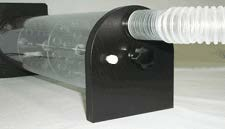
\includegraphics[width=0.6\textwidth]{../images/PF_II_2.jpg}
	\caption{Inlet of Gas-System2 connected to AFT7 tubing}
	\label{inlet}
	\end{figure}
	
	\item Assemble airflow accessories and connect them to the gas chamber. Keep in mind that some of these components might already be assembled (Fig. \ref{airflow}).\begin{enumerate}
	\item Attach your disposable bacteriological filter (AFT1) to inlet side of the airflow transducer (SS11LA).
	\item Connect AFT22 T-valve to opposite side of airflow transducer. Check that the arrows indicating airflow are pointing away from the airflow transducer.
	\item Connect AFT11C couplers to remaining two ports of T-valve.
	\item Use AFT11E (blue coupler) to connect AFT7 tubing to T-valve in the port opposite of SS11LA connection.
	\item Attach AFT6 calibration syringe to remaining port of T-valve.
	\end{enumerate}
	
	\begin{figure}[h]
	\centering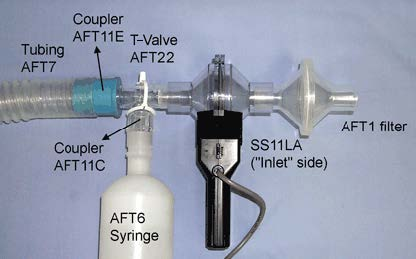
\includegraphics[width=0.6\textwidth]{../images/PF_II_3.jpg}
	\caption{Schematic of airflow accessories connected to Gas-System2}
	\label{airflow}
	\end{figure}
	
	\item Connect SS11LA airflow transducer to channel 1.
	\item Connect O\textsubscript{2} output from Gas-System2 to channel 2.
	\item Connect CO\textsubscript{2} output from Gas-System2 to channel 3.
	\item Turn on MP3X.
\end{enumerate}

\subsection*{Calibration}
\begin{enumerate}
	\item Open BIOPAC student lab lessons software and select \textit{H19 - VO2 and RER} (located under PRO lessons).
	\item Pump calibration syringe 15-20 times to flush Gas-System2 chamber with ambient air.
	\item Select \textit{MP3X} from the menu bar at the top of the screen, then choose \textit{Set Up Data Acquisition}.
	\item Make sure the sampling rates of all three channels are set to 100 Hz. Check all boxes (Acquire, Plot, and Value) for channels 1, 2, and 3. 
	
	\item Calibrate airflow (channel 1).\begin{enumerate}
	\item Select row 1 (Airflow) and click \textit{Setup} in the top right corner of the window.
	\item Click \textit{Scaling} at the bottom of the pop up window.
	\item Hold airflow transducer still and upright and press \textit{Cal 1} button.
	\item Subtract 3000 from \textit{Cal 1} value and enter as \textit{Cal 2} input value field.
	\item Check \textit{Cal 1} Map value is zero and \textit{Cal 2} value is 10.
	\item Click \textit{OK} twice to exit.
	\end{enumerate}
	
	\item Calibrate O\textsubscript{2} (channel 2).
	\begin{enumerate}
		\item Select row 2 (O2e) and click \textit{Setup} in the top right corner of the window.
	\item Click \textit{Scaling} at the bottom of the pop up window.
	\item Click on \textit{Cal 2} button.
		\item Enter value 20.93 as \textit{Cal 2} Map value.
		\item Confirm that both \textit{Cal 1} input value and \textit{Cal 1} Map value are zero.
	\item Click \textit{OK} twice to exit.
	\end{enumerate}
	
	\item Calibration CO\textsubscript{2} (channel 3).
	\begin{enumerate}
		\item Select row 3 (CO2e) and click \textit{Setup} in the top right corner of the window.
	\item Click \textit{Scaling} at the bottom of the pop up window.
	\item Click on \textit{Cal 1} button.
		\item Enter value 0.04 as \textit{Cal 1} Map value.
		\item Add 10 to \textit{Cal 1} input value and enter as \textit{Cal 2} input value.
		\item Set \textit{Cal 2} scale value to 1.04.
	\item Click \textit{OK} twice to exit.
	\end{enumerate}
\end{enumerate}

\subsection*{Test Procedure}
\subsubsection*{General Guidelines}
\begin{enumerate}
	\item Before every trial, pump calibration syringe 15-20 times to flush the mixing chamber with ambient air.
	\item While recording, hold airflow apparatus very still parallel to floor. Make sure to keep the airflow transducer handle perpendicular to floor.
	\item Begin every recording with inhalation and end with exhalation. This will prevent receiving O\textsubscript{2} inspiration values less that that of total expiration.
	\item Record for a few seconds without breathing at the beginning of each experiment to ensure that the baselines are correct. Hit the vertical autoscale button, as needed, to confirm the magnitude of the baseline traces. If baseline values are not correct, stop and troubleshoot.
	\item Replace calibration syringe with AFT1 filter and AFT2 mouthpiece (Fig. \ref{syringe}).
	\begin{figure}[h]
	\centering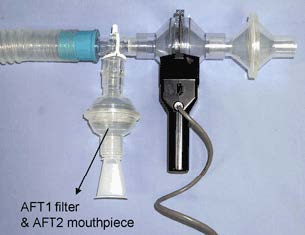
\includegraphics[width=0.6\textwidth]{../images/PF_II_8.jpg}
	\caption{Schematic of airflow accessories with AFT1 filter and AFT2 mouthpiece}
	\label{syringe}
	\end{figure}
\end{enumerate}

The output from the BIOPAC Pro Software is summarized in Table \ref{abbreviation}.

\begin{table}[h]
	\centering
	\caption{BIOPAC Pro Software output}
	\begin{tabular}[h!]{p{0.5\textwidth}|p{0.15\textwidth}|p{0.15\textwidth}}
	\toprule
	Output & Abbreviation & Units\\
	\midrule
	Airflow through the pneumotachometer & Airflow & [L/sec]\\
	O\textsubscript{2} concentration in the mixing chamber & O2E (expired) & [volume \%]\\
	CO\textsubscript{2} concentration in the mixing chamber & CO2E (expired) & [volume \%]\\
	Volume of O\textsubscript{2} consumed at STP per 60 sec interval & VO2* & [L/min]\\
	Respiratory Exchange Ratio & RER & [-]\\
	\bottomrule
	\end{tabular}
	\label{abbreviation}
	\end{table}

\subsection*{Test Procedure}
\subsubsection*{Normal Breathing}
\begin{enumerate}
	\item Have the subject put a nose clip on.
	\item Press Start button in the lower right corner of the Pro Software.
	\item Record for a few seconds without breathing to ensure the baselines are correct.
	\item Have the subject breathe normally in and out of the mouthpiece for at least 2 minutes. This ensures that mixing occurs and that the tank fills completely with exhaled air.
	\item Press the Stop button in the Pro Software and save your data.
\end{enumerate}

\subsubsection*{Hyperventilation}
\begin{enumerate}
	\item Have the subject put a nose clip on.
	\item Press Start button in lower right corner of the Pro Software.
	\item Record for a few seconds without breathing to ensure the baselines are correct.
	\item Have the subject breathe normally for 1 minute.
	\item Have the subject hyperventilate for 1 minute.
	\item Resume normal breathing for 1 minute.
	\item Press the Stop button in the Pro Software and save your data.
\end{enumerate}

\subsubsection*{Recovery from Exercise}
\begin{enumerate}
	\item Perform the exercise of your choice that gets your heart rate up.
	\item Following exercise, immediately attach nose clip.
	\item Press Start button in lower right corner of the Pro Software.
	\item Record for a few seconds without breathing to ensure the baselines are correct.
	\item Breathe in an out of the mouthpiece for at least 2 minutes.
	\item Press the Stop button in the Pro Software and save your data.
\end{enumerate}

\section*{Data Analysis}

Use the following values, if necessary:\begin{itemize}
	\item Ambient air composition by volume: 20.93\% O\textsubscript{2}, 0.04\% CO\textsubscript{2}, 79.03\% N\textsubscript{2}
	\item Vapor pressure of water is 22.4 mmHg and 75\degree F and 47.07 mmHg at 98.6\degree F
\end{itemize}

\begin{enumerate}
	\item Complete the chart for O\textsubscript{2} \%, CO\textsubscript{2} \%, and VO\textsubscript{2} over the three test conditions.
	\item Complete the chart for molar concentrations of O\textsubscript{2} over the listed conditions.
	\item Compare and explain the results. Focus on comparisons between A \& B, B \& C, D \& E, and B \& E.
	\item For each of the three test conditions, determine the mean measured breathing or respiratory rate and the tidal volume. \textit{Hint}: obtain tidal volume from the airflow trace.
	\item Explain your method for determining the breathing rate and the tidal volume.
	\item Based on your data, how many moles of O\textsubscript{2} are consumed per breath for normal breathing? How many moles of CO\textsubscript{2} are produced per breath for normal breathing? The volume of the mixing chamber is 5 L. Record these numbers for the post-lab.
	\item Calculate the pulmonary ventilation rate for each of the three conditions through the following steps:\begin{enumerate}
	\item Calculate the minute respiratory rate (total pulmonary ventilation rate) and record in the chart below. Explain how you performed the calculation.
	\item Compare and briefly explain differences in minute respiratory rate among the test conditions.
	\item Calculate the alveolar ventilation rate and record in the chart below. Assume a dead space volume of 150 mL/breath. Explain how you performed the calculation.
	\item Compare and briefly explain differences in alveolar ventilation rate among the test conditions. Use the dead space of 150 mL to fill in the table.
	\item Which of the two ventilation rates is a more accurate indicator of the efficiency of actual breathing/ventilation? Explain.
	\end{enumerate}
	
	\item The rate of oxygen consumption is equal to the rate of oxygen diffusion across the respiratory membrane. Determine the rate of oxygen consumption for the normal and exercise conditions based on your experimental data.
	\item How do the measured O\textsubscript{2} consumption rates at rest and after exercise compare?
\end{enumerate}
\end{document}
